\section*{Experiment 1: To familiarize students with some basic components like resistor, capacitor, inductor, diode, transistor, some basic logic ICs, breadboard, etc.}  
\addcontentsline{toc}{section}{Experiment 1: To familiarize students with some basic components like resistor, capacitor, inductor, diode, transistor, some basic logic ICs, breadboard, etc.}


\subsection*{Resistors}

A resistor is a passive two-terminal electrical component that implements electrical resistance as a circuit element. The current through a resistor is in direct proportion to the voltage across the resistor's terminals. This relationship is represented by Ohm's law. It is a device used in electrical circuits to maintain a constant relation between current flow and voltage. 

\begin{figure}[H]
    \centering
    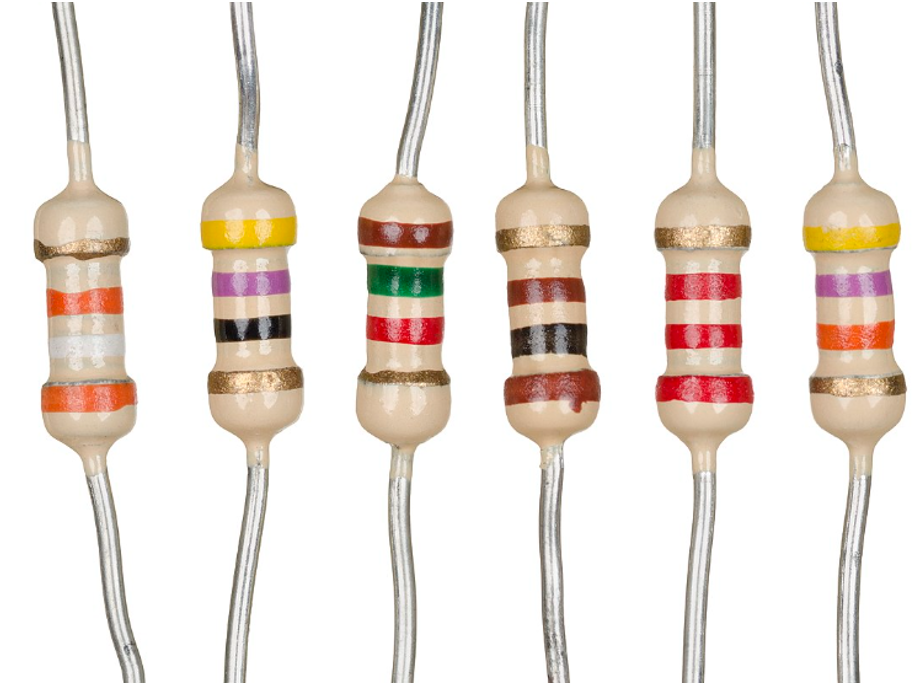
\includegraphics[width=0.5\linewidth]{img/resistor.png}
    \caption{Resistors of different values}
    \label{fig:resistor}
\end{figure}

\noindent \textbf{Circuit Diagram}

\begin{center}
    \begin{circuitikz}
        % Fixed Resistor
        \draw (0,0) to[resistor] (2,0);
        \node at (1,-0.7) {Fixed Resistor};
        
        % Variable Resistor
        \draw (4,0) to[variable resistor] (6,0);
        \node at (5,-0.7) {Variable Resistor};
    \end{circuitikz}
\end{center}

\noindent \textbf{Resistor Color Code}

\noindent The resistance value and tolerance of resistors are usually indicated by color coding. Color bands are printed on the body. They consist of four color bands or 5 color bands \& they are read from left to right. A typical resistor with color bands is shown in figure 

\begin{figure}[H]
    \centering
    \includesvg[width=0.5\linewidth]{img/resistor_color_code.svg}
    \caption{Values of resistors can be determined using their color code}
    \label{fig:colorcode}
\end{figure}

\noindent The above resistor has 4 color bands. The first band represents the first digit. The second band represent second digit The third band represent multiplier (this gives the no. of zeros after the 2 digits) The 4th band represents tolerance in \% 

\vspace{1 cm}
\noindent \textbf{The color codes are presented in below table}

\begin{table}[H]
    \centering
    \renewcommand{\arraystretch}{1.2}
    \setlength{\tabcolsep}{8pt}
    
    \begin{tabular}{c| m{2.5cm} |m{2.5cm}|m{2.5cm}|m{2.5cm}}
    \hline
        Color & First Digit for the 1st Band &  Second Digit for the 2nd Band & Multiplier Digit for the 3rd Band & Resistance Tolerance\\
    \hline \hline    
        Black & 0 & 0 & $10^0$ & - \\
        Brown & 1 & 1 & $10^1$ & $\pm 1\%$\\
        Red & 2 & 2 & $10^2$  & $\pm 2\%$ \\
        Orange & 3 & 3 & $10^3$ & $\pm 3\%$ \\ 
        Yellow & 4 & 4 & $10^4$ & - \\ 
        Green & 5 & 5 & $10^5$ & - \\
        Blue & 6 & 6 & $10^6$ & - \\ 
        Violet & 7 & 7 & $10^7$ & - \\
        Gray & 8 & 8 & $10^8$ & - \\ 
        White & 9 & 9 & $10^9$ & - \\ 
        Gold & - & - & $10^{-1}$ & $\pm 5\%$ \\
        Silver & - & - & $10^{-2}$ & $\pm 10\%$ \\
        No Color & - & - & - & $\pm 20\%$ \\
        
    \hline 
    \end{tabular}

    \label{tab:my_label}
\end{table}

\noindent \textbf{N.B.} The resistance value can also be measured directly using a Multimeter

\vspace{1 cm}
\noindent \textbf{Example} 

\noindent The resistor has a color band sequence green, blue, brown and silver. Identify the resistance value.


\begin{figure}[H]
    \centering
    \includesvg[width=0.5\linewidth]{img/resistor_example}
    \label{fig:example}
\end{figure}

\begin{table}[H]
    \centering
    \begin{tabular}{c|c|c|c}
    \hline
        1st Band &  2nd Band & 3rd Band & 4th Band\\
    \hline \hline    
        1st Digit & 2nd Digit & Multiplier & Tolerance \\
        5 & 6 & $10^1$ & $\pm 10\%$ \\
    \hline 
    \end{tabular}

    \label{tab:my_label}
\end{table}

\noindent The resistance value = $56 \times 10^1 \pm 10\% = 560 \Omega \ \pm 10\%$ 

\noindent Therefore the resistance should be within the range $555 \Omega$ to $565 \Omega$

\subsection*{Capacitors}

Capacitors can store energy in the electric field located between plates. They are commonly used in electronic circuits for storage. They can also be used in filter circuits to differentiate between high and low-frequency signals. Capacitors can be majorly classified into Ceramic Capacitors, Electrolytic Capacitors, Mylar capacitors etc.

\begin{figure}[H]
    \centering
    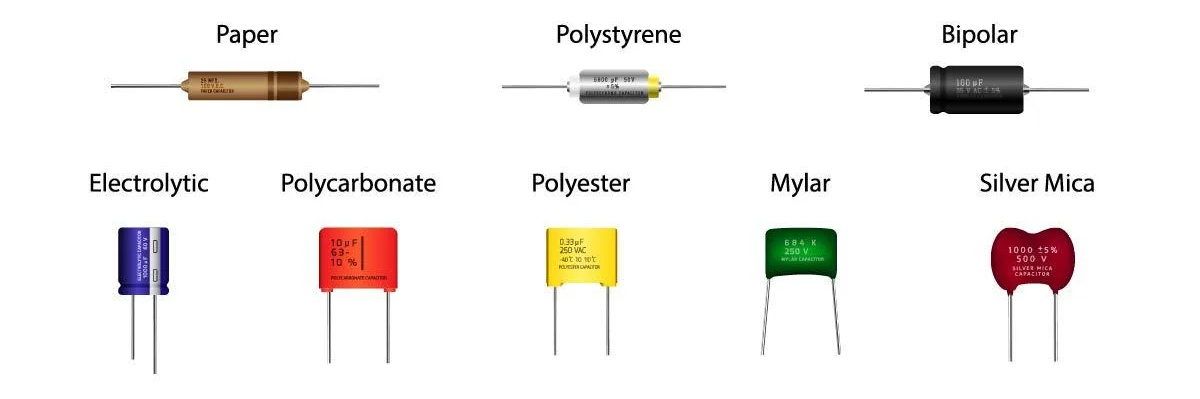
\includegraphics[width=0.9\linewidth]{img/capacitor.png}
    \caption{Different types of capacitors}
    \label{fig:enter-label}
\end{figure}


\subsection*{Inductors}

An inductor, also called a coil or reactor, is a passive two-terminal electrical component which resists changes in electric current passing through it. It consists of a conductor such as a wire, usually wound into a coil. When a current flows through it, energy is stored in a magnetic field in the coil. When the current flowing through an inductor changes, the time-varying magnetic field induces a voltage in the conductor, according to Faraday’s law of electromagnetic induction, which by Lenz's law opposes the change in current that created it. 

\vspace{0.25cm}

\noindent Inductors, also called coils, can be a bit harder to figure out their values. If they are color coded, the resources listed for resistors can help, otherwise a good meter that can measure inductance will be needed.

\begin{figure}[H]
    \centering
    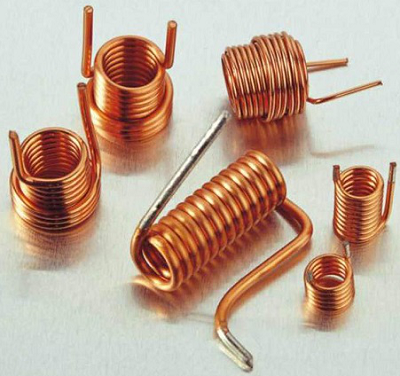
\includegraphics[width=0.4\linewidth]{img/inductor.jpg}
    \caption{Inductors}
    \label{fig:inductors}
\end{figure}

\subsection*{Diode}

In electronics, a diode is an active two-terminal electronic component with unidirectional conductance, it has low (ideally zero) resistance to current flow in one direction, and high (ideally infinite) resistance in the other.

\begin{figure}[H]
    \centering
    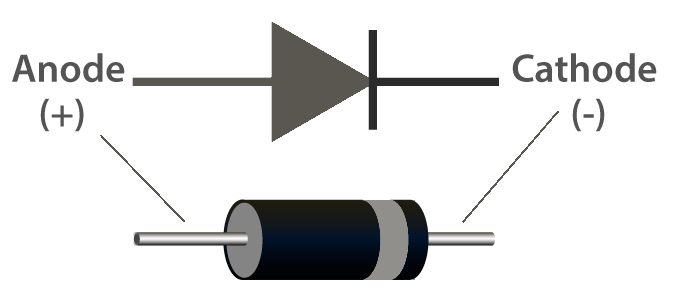
\includegraphics[width=0.5\linewidth]{img/diode.png}
    \caption{Diode and it's circuit symbol is shown at the top}
    \label{fig:diode}
\end{figure}

\subsection*{Transistors}

A transistor is a semiconductor device used to amplify and switch electronic signals and electrical power. It is composed of semiconductor material with at least three terminals for connection to an external circuit. A voltage or current applied to one pair of the transistor's terminals changes the current through another pair of terminals. Because the controlled (output) power can be higher than the controlling (input) power, a transistor can amplify a signal. The most popular and commonly used transistors are \verb|BC547|, \verb|2N2222|, and \verb|BC557|.

\begin{figure}[H]
    \centering
    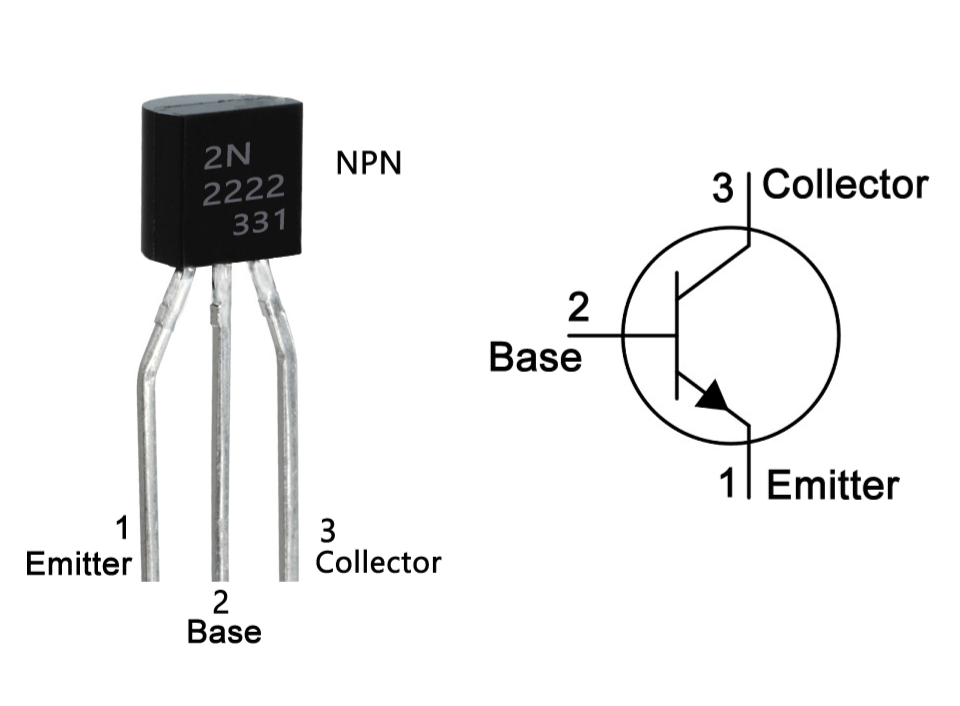
\includegraphics[width=0.5\linewidth]{img/transistor.png}
    \caption{ 2N222A pin configuration and symbol}
    \label{fig:transistor}
\end{figure}

\subsection*{Basic Logic Gates ICs}

An integrated circuit or monolithic integrated circuit (also referred to as an IC, a chip, or a microchip) is a set of electronic circuits on one small plate ("chip") of semiconductor material, normally silicon.

\vspace{0.25 cm}

\noindent Digital electronics rely on the actions of just seven types of logic gates, called AND, OR, NAND (Not AND), NOR (Not OR), XOR (Exclusive OR) XNOR (Exclusive NOR) and NOT. These can be implemented using the following IC pin diagrams.

\begin{figure}[H]
    \centering
    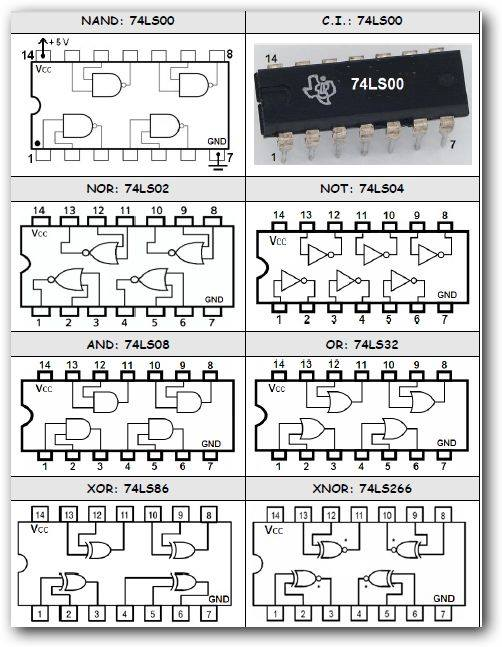
\includegraphics[width=0.75\linewidth]{img/logic_gates.jpg}
    \caption{Different logic gates}
    \label{fig:enter-label}
\end{figure}

\subsection*{Breadboard}

The breadboard has two basic internal connections, the vertical and horizontal. The verticals are connected from top to bottom, if 5 volts is placed on the very first pin, 5 volts will be present at the very last pin and any pin in between; this is demonstrated in Figure 1.2 from red pin to red pin. The horizontal strips are connected by every 5 pins. Looking at Figure 1.3 pin A1 to E1 are connected internally. 

\begin{figure}[H]
    \centering
    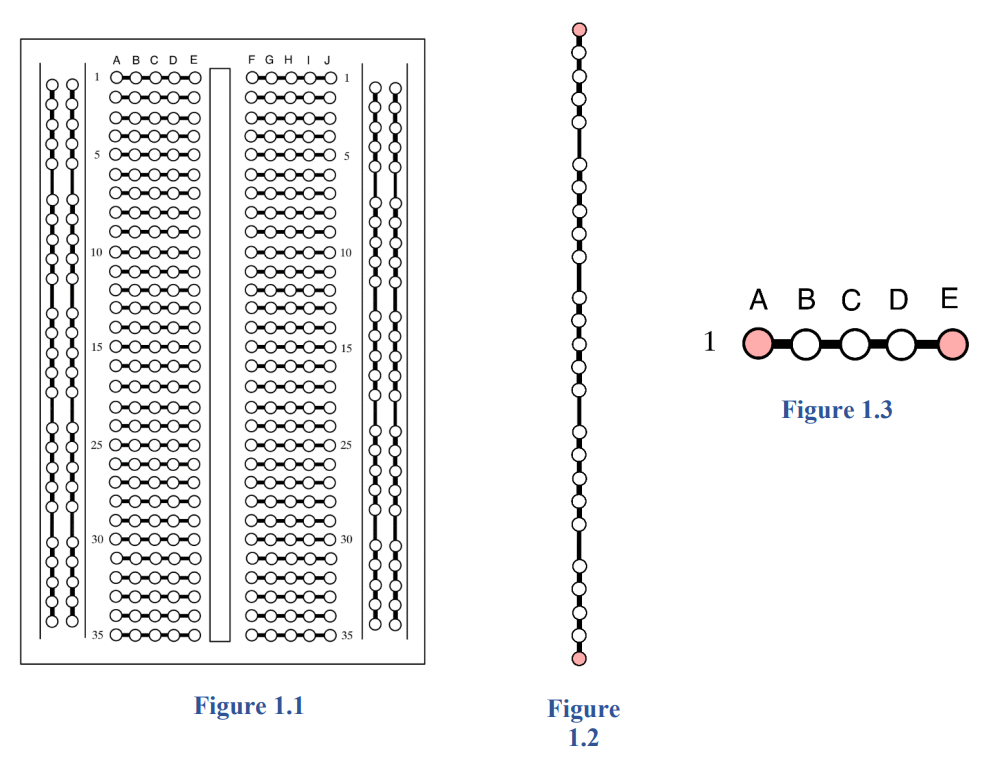
\includegraphics[width=1\linewidth]{img/breadboard.png}
    \label{fig:breadboard}
\end{figure}

\newpage
